
\section{Ap\^endice - Modelos ARIMAX, SARIMA e SARIMAX }\label{sec:arimaxsarimasarimax24}

\begin{figure}[H]
	\centering
	\caption{Comparação dos modelos ARIMAX, SARIMA e SARIMAX, 1 dia à frente }
	\label{fig:1-ARIMAX-SARIMA-SARIMAX24}
	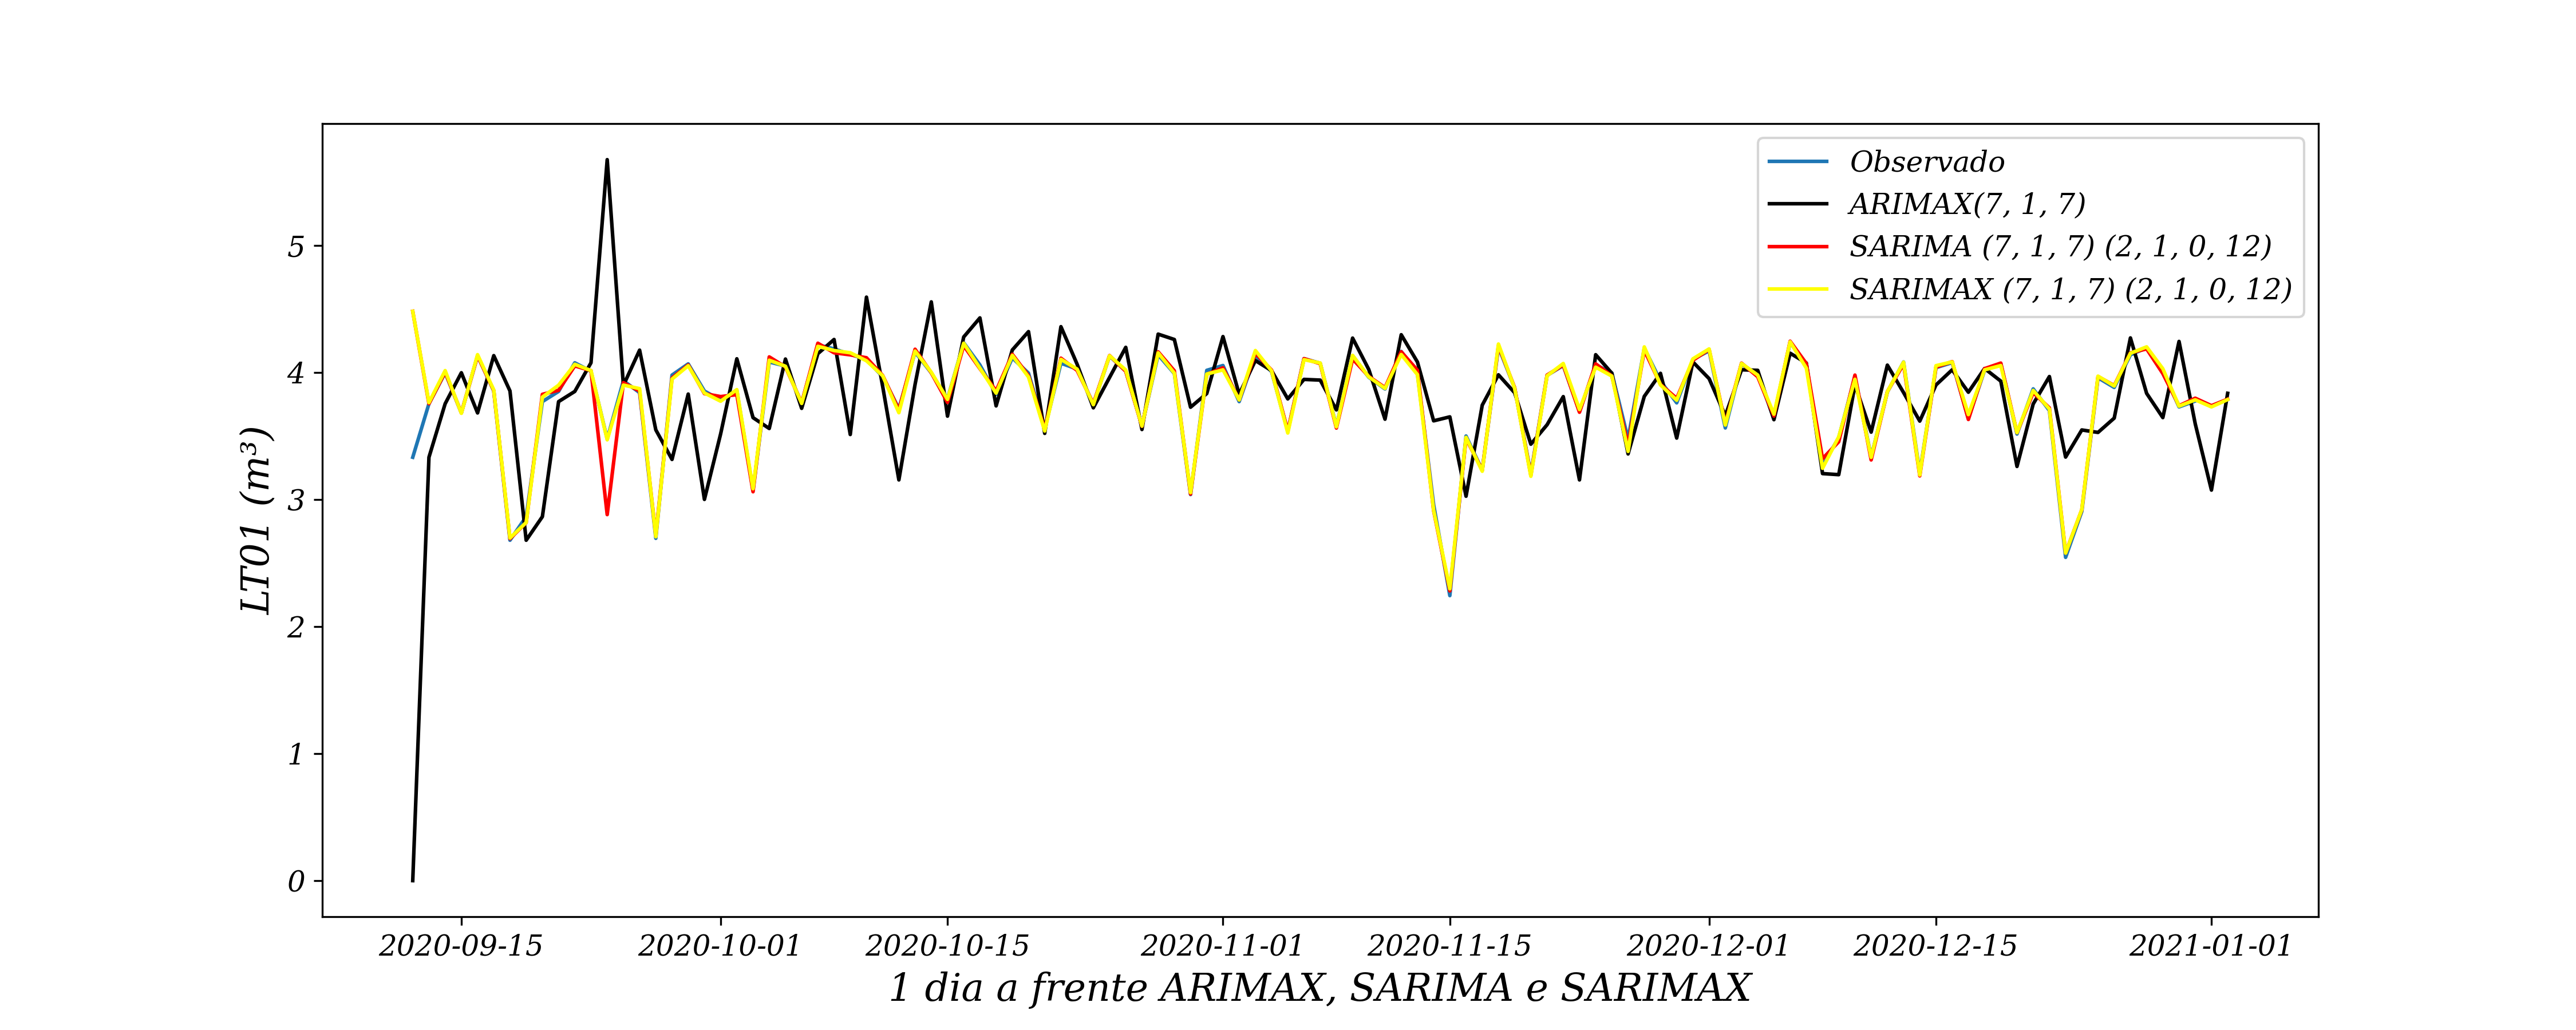
\includegraphics[width=1\linewidth]{Apendices/Figuras/modelagem-24h/1-ARIMAX-SARIMA-SARIMAX}
	
		\fonte{Elaboração própria a partir de dados da SANEPAR (2018 a 2020)}
\end{figure}

\begin{figure}[!htb]
	\centering
	\caption{Comparação dos modelos ARIMAX, SARIMA e SARIMAX, 7 dias à frente }
	\label{fig:10-ARIMAX-SARIMA-SARIMAX24}
	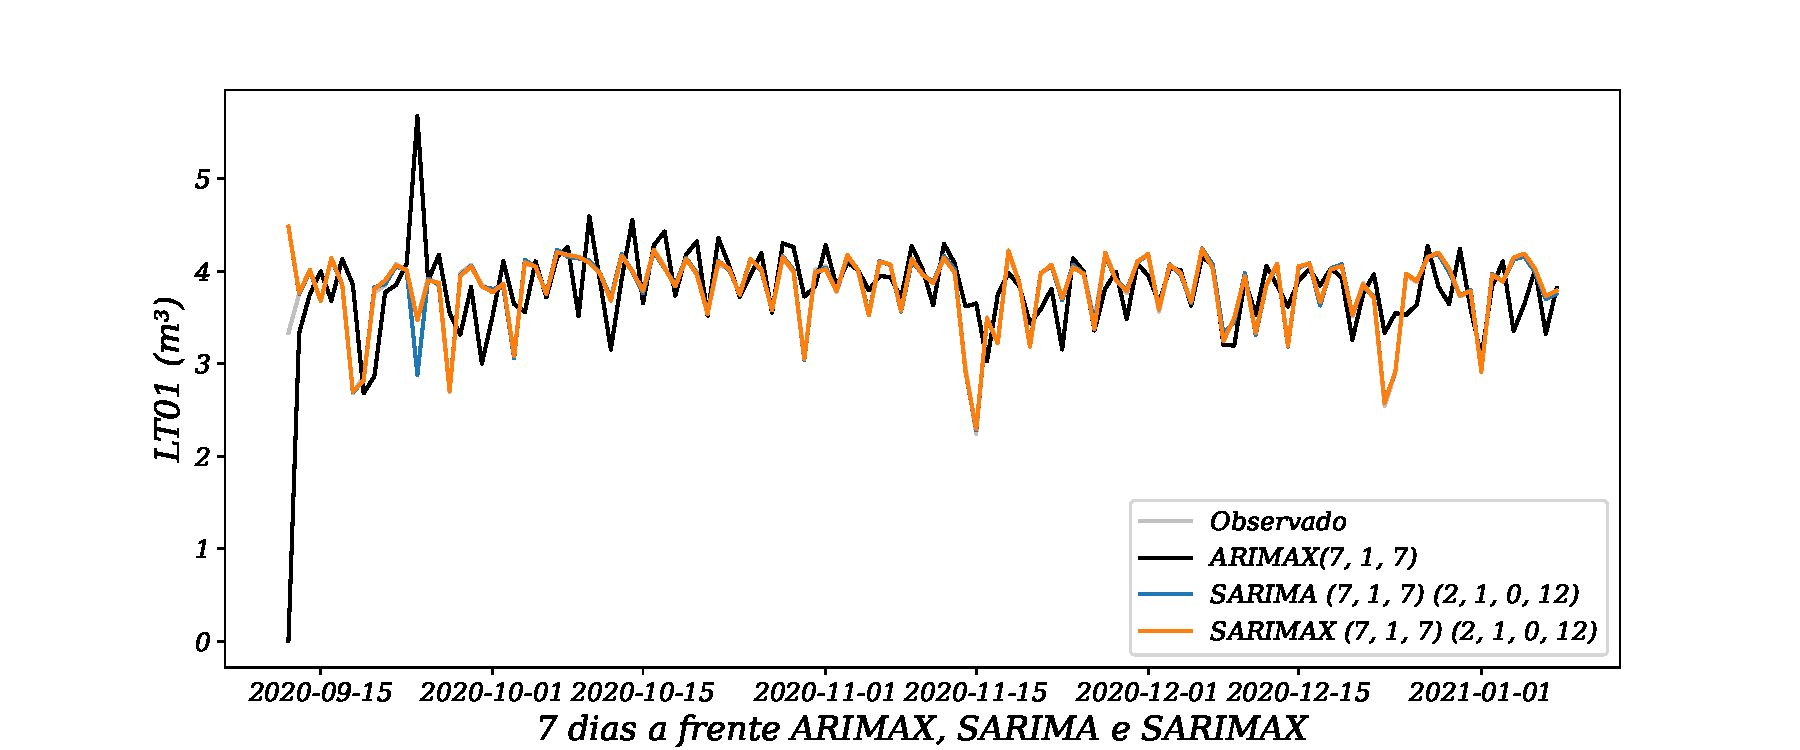
\includegraphics[width=1\linewidth]{Apendices/Figuras/modelagem-24h/7-ARIMAX-SARIMA-SARIMAX}
	
	\fonte{Elaboração própria a partir de dados da SANEPAR (2018 a 2020)}
\end{figure}


\begin{figure}[H]
	\centering
	\caption{Comparação dos modelos ARIMAX, SARIMA e SARIMAX, 14 dias à frente }
	\label{fig:30-ARIMAX-SARIMA-SARIMAX24}
	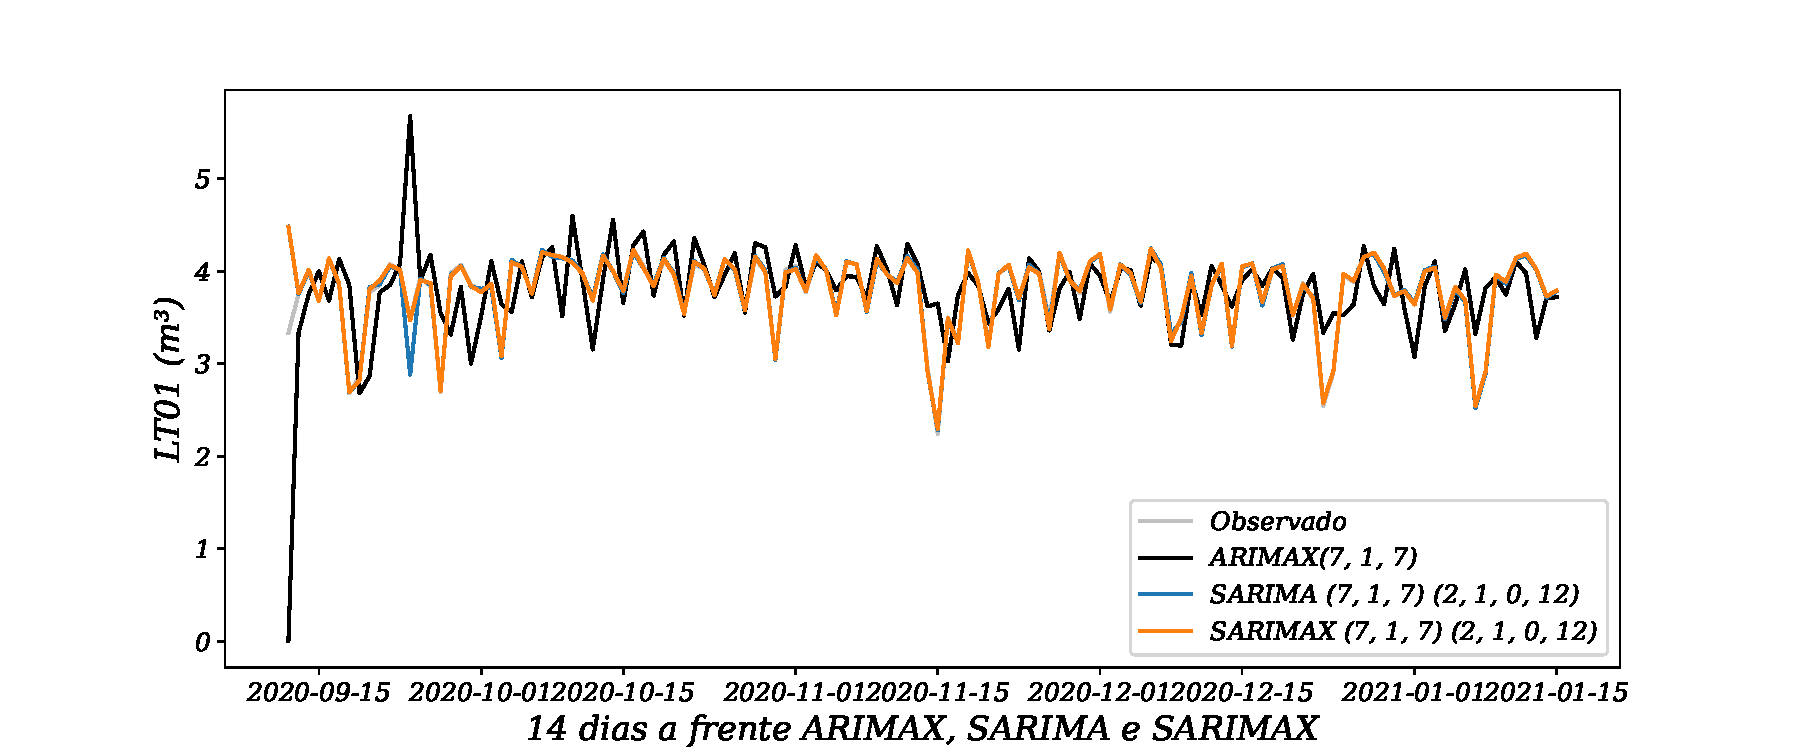
\includegraphics[width=1\linewidth]{Apendices/Figuras/modelagem-24h/14-ARIMAX-SARIMA-SARIMAX}
	
	\fonte{Elaboração própria a partir de dados da SANEPAR (2018 a 2020)}
\end{figure}

\begin{figure}[!htpb]
	\centering
	\caption{Comparação dos modelos ARIMAX, SARIMA e SARIMAX, 30 dias à frente }
	\label{fig:60-ARIMAX-SARIMA-SARIMAX24}
	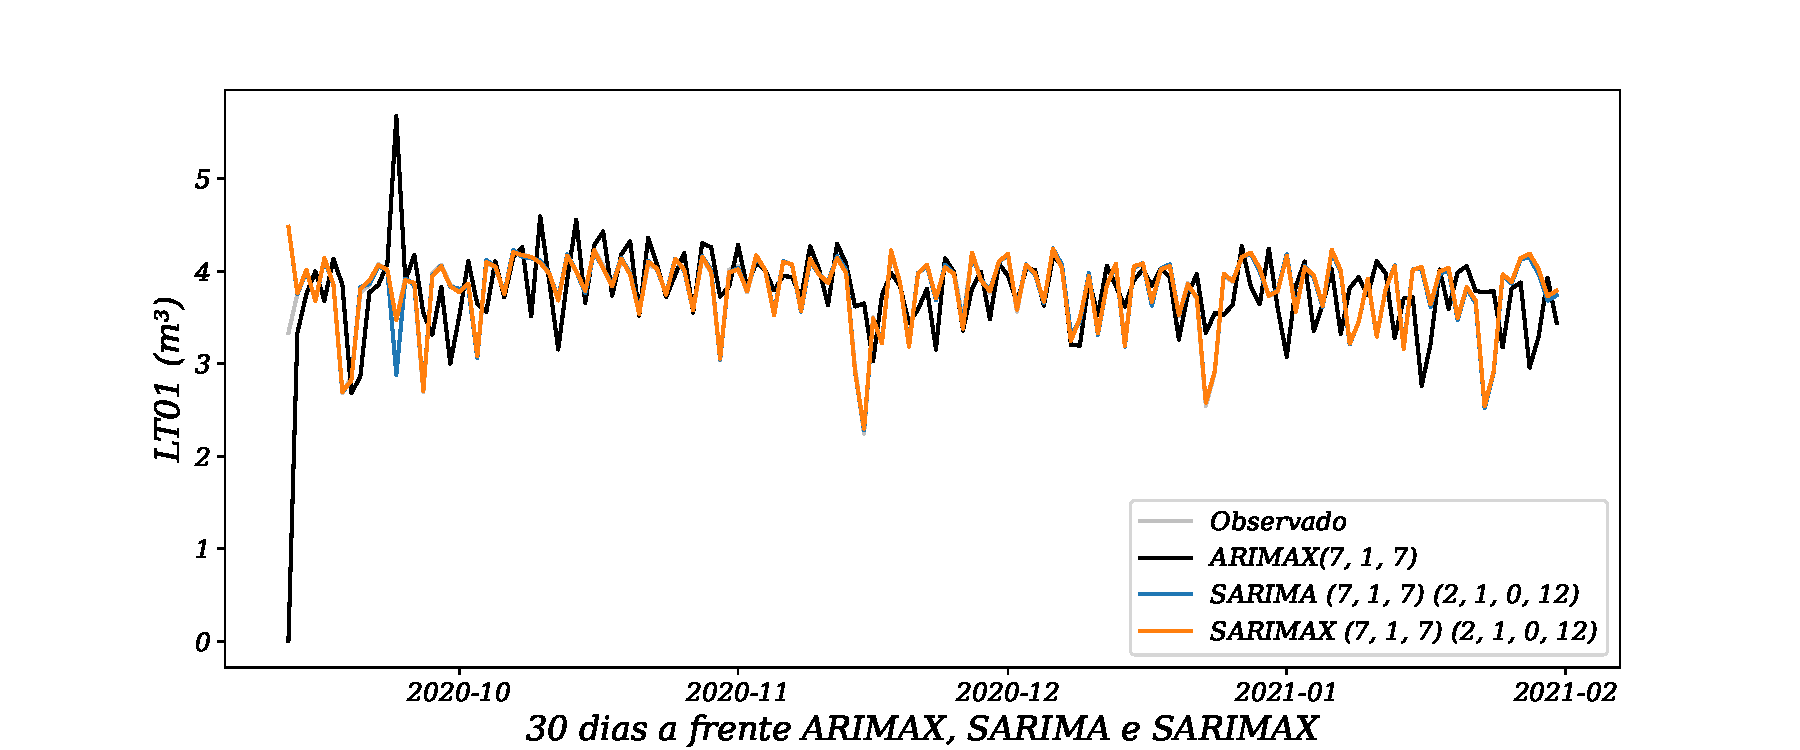
\includegraphics[width=1\linewidth]{Apendices/Figuras/modelagem-24h/30-ARIMAX-SARIMA-SARIMAX}
	
	\fonte{Elaboração própria a partir de dados da SANEPAR (2018 a 2020)}
\end{figure}

\newpage

\section{Ap\^endice - Modelos RNN e Prophet }\label{sec:rnnprophet}

\begin{figure}[!htpb]
	\centering
	\caption{A rede neural recorrente (RNN) com todos os horizontes }
	\label{fig:rnn}
	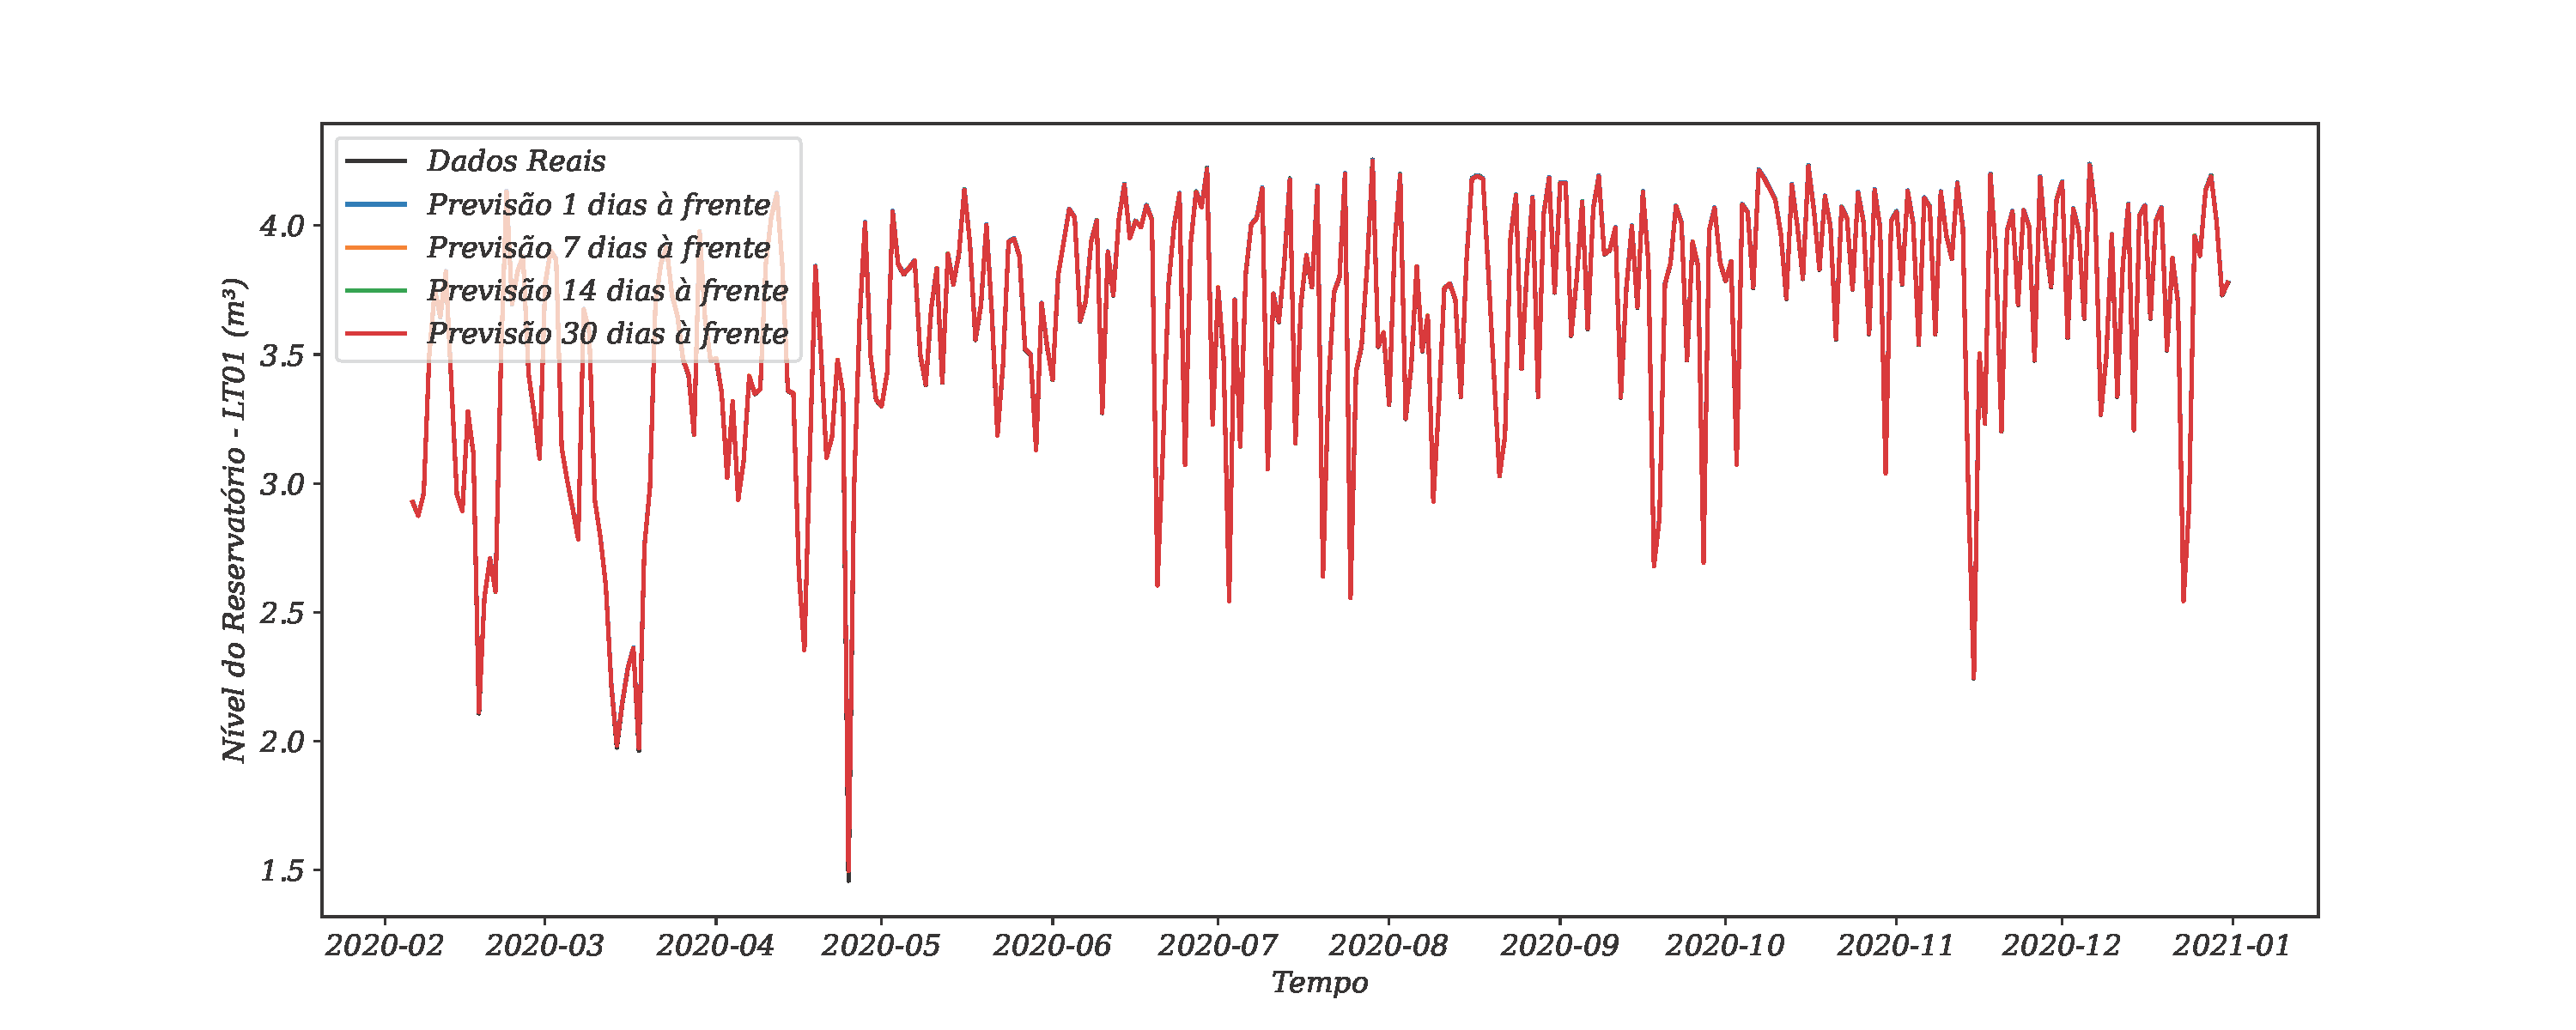
\includegraphics[width=1\linewidth]{Apendices/Figuras/modelagem-24h/RNN}
	
	\fonte{Elaboração própria a partir de dados da SANEPAR (2018 a 2020)}
\end{figure}

\begin{figure}[!htpb]
	\centering
	\caption{Previsões do Modelo Prophet para Diferentes Horizontes}
	\label{fig:prophet}
	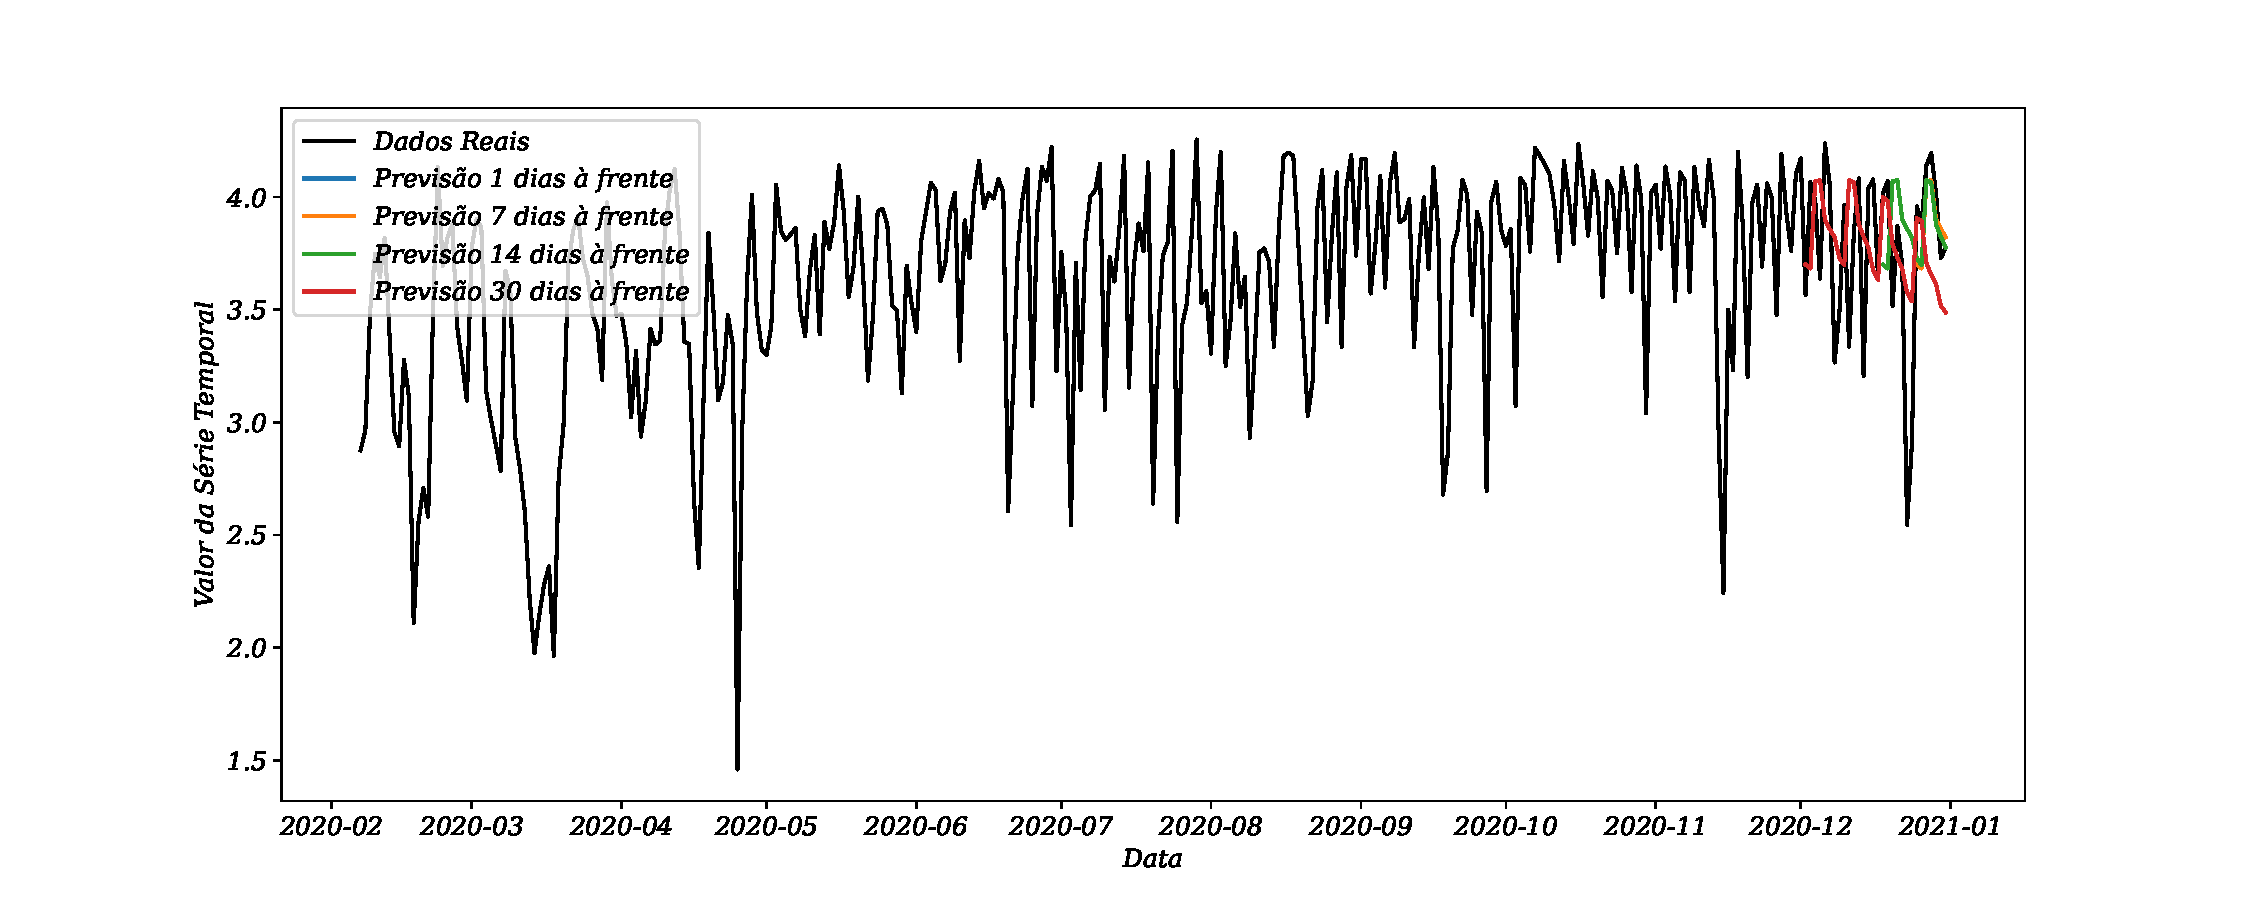
\includegraphics[width=1\linewidth]{Apendices/Figuras/modelagem-24h/prophet}
	
	\fonte{Elaboração própria a partir de dados da SANEPAR (2018 a 2020)}
\end{figure}